\documentclass[a4paper,11pt]{article}
\usepackage[T1]{fontenc}
\usepackage[utf8]{inputenc}
\usepackage{lmodern}
\usepackage{textcomp}
\usepackage{amssymb}
\usepackage[margin=1.5cm]{geometry}

\title{HICF1 ATM mutation and VAF}
\author{Dr. Susanne Weller}
\date{\today}

\usepackage{Sweave}
\begin{document}
\maketitle
\section*{Disclaimer}
This analysis is still preliminary! Do not use graphs or p-values for presentations, poster or reports!
\section*{Objectives}
The purpose of this analysis is to describe how mutations in ATM occur at different Variant Allele Frequencies (VAF). Some patients have more than one mutation, and these mutations differ in their VAF. We want to know if we can see two distinctive groups in VAF in those patients.

\section*{Mutation Distribution}
This illustrates how many samples have more than one mutation:\\
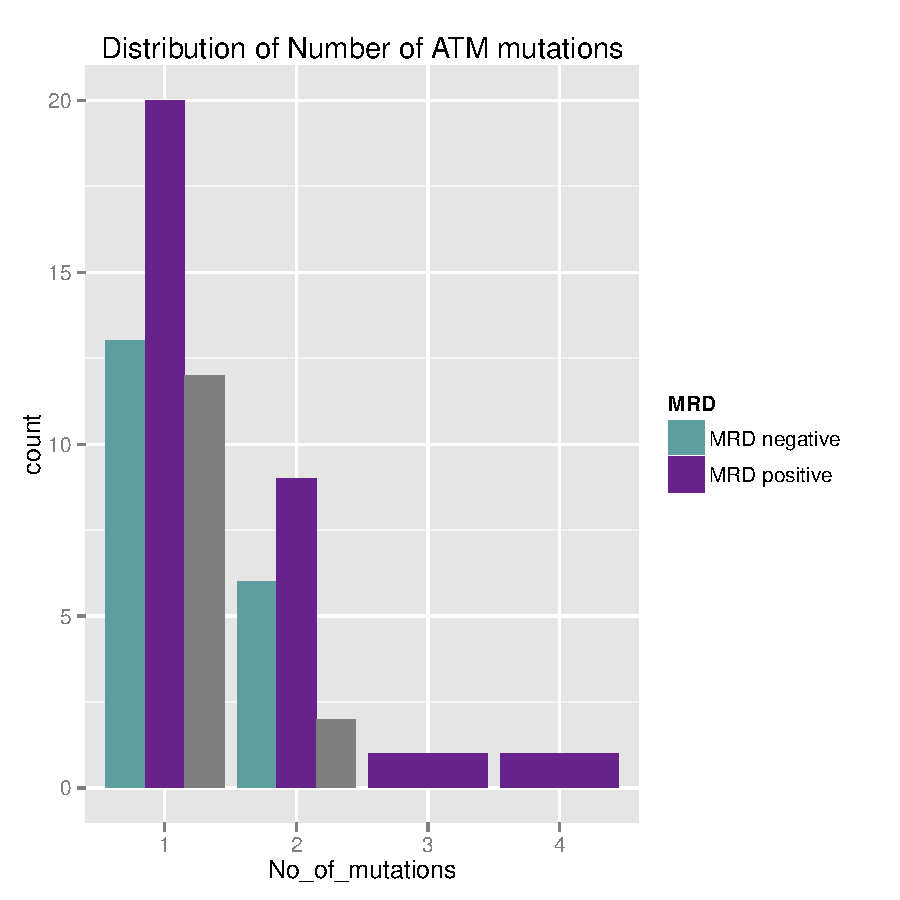
\includegraphics{ATM_VAF-002}
\\I added all patients that have more than one mutation because there are only 2 of them and two groups is usully easier to deal with:\\
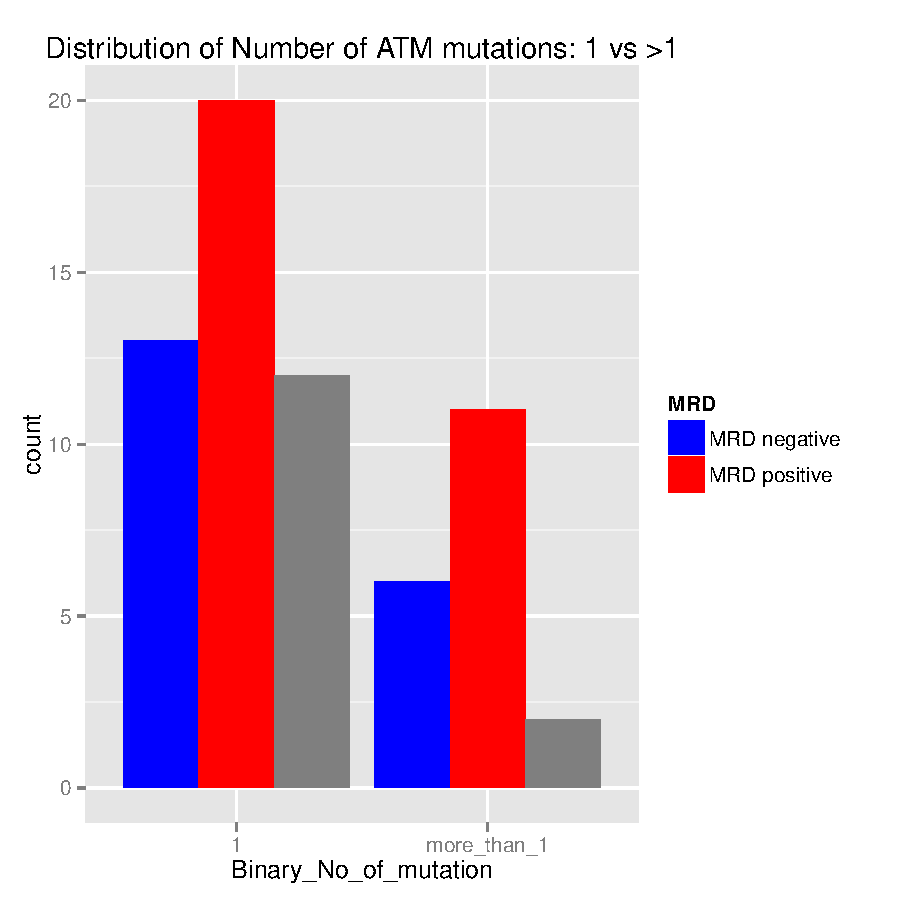
\includegraphics{ATM_VAF-003}
\\If you look at it from the perspective of clinical outcome (MRD):\\
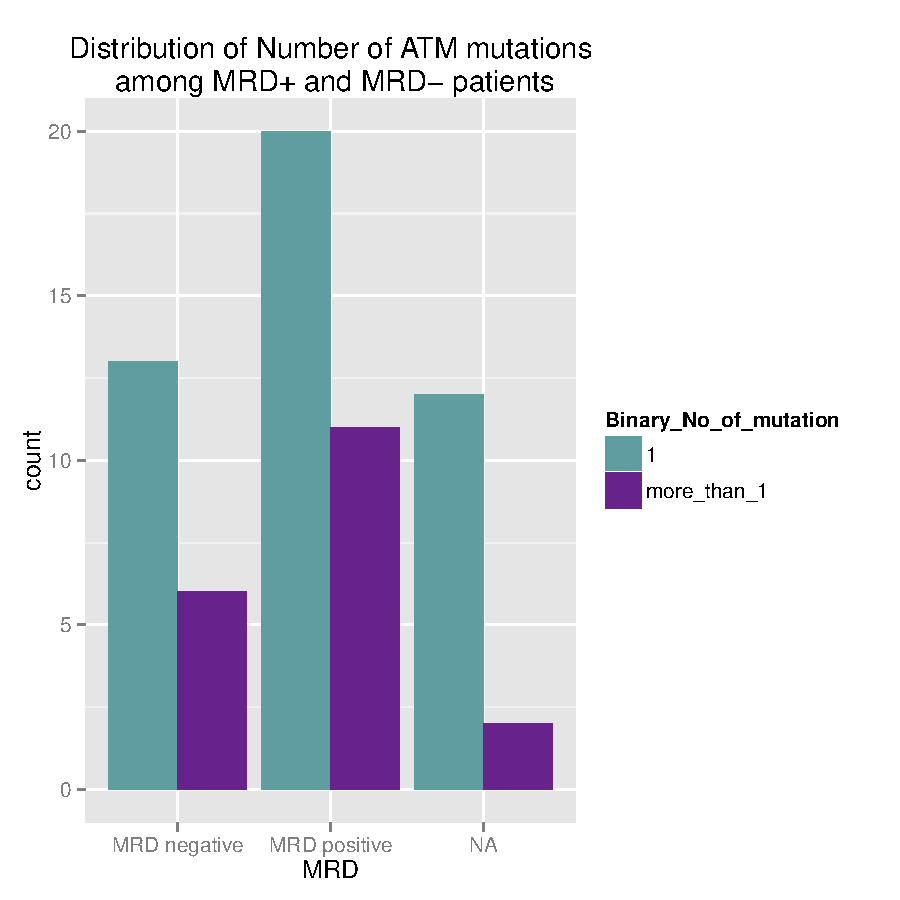
\includegraphics{ATM_VAF-004}
\\We can check if the distribution of Number of mutations between MRD positive and negative is different:\\
\begin{Schunk}
\begin{Soutput}
                1 more_than_1
  MRD negative 13           6
  MRD positive 20          11
\end{Soutput}
\begin{Soutput}
	Pearson's Chi-squared test with Yates' continuity correction

data:  Mutationdistribution
X-squared = 0, df = 1, p-value = 1
\end{Soutput}
\end{Schunk}
\\Apparently, MRD negative and MRD positive patients do not differ in their distribution of ATM mutation numbers. Next, we look at the the distribution of the actual VAF:\\
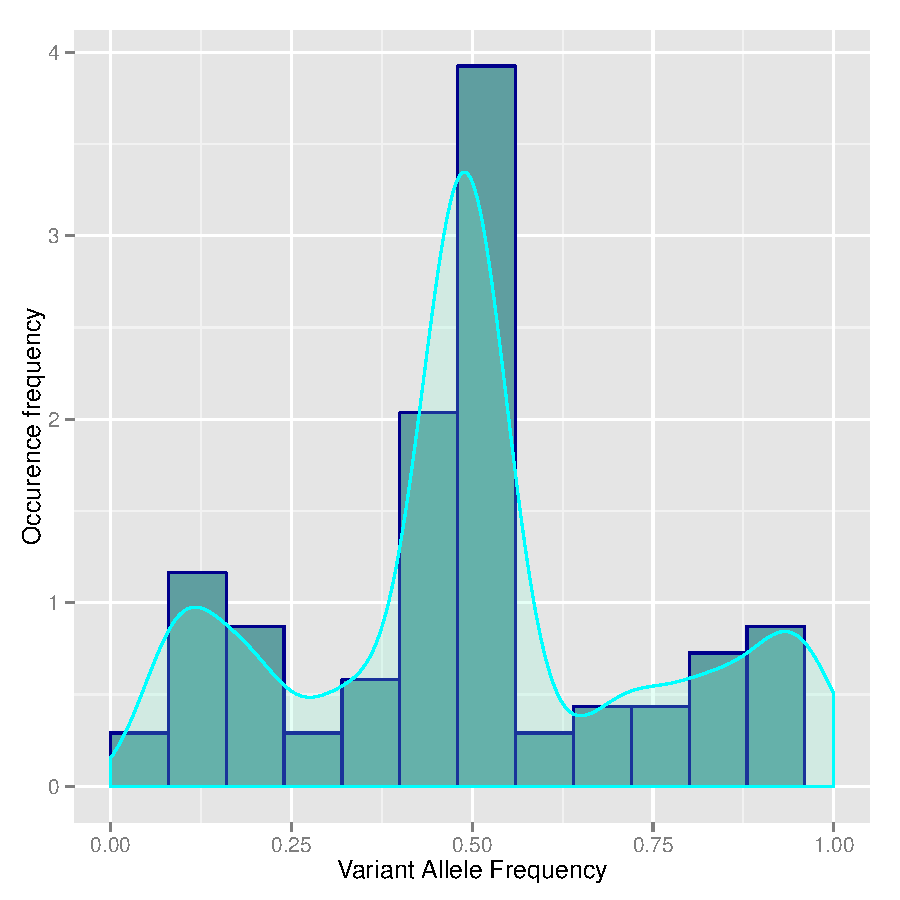
\includegraphics{ATM_VAF-006}
\\Notice how most mutations have a VAF around 0.5, but there are two local maxima closer to both ends of the spectrum. We want to know wheather those correspond to patients that have more than one mutation. Keep in mind that this graph illustrates all VAFs, so 17 patients occure in it more than once!\\
\section*{Clustering of Variant Allele Frequencies}
First, we have a look at the VAF distribution of patients with 1,2, 3 or 4 mutations. Again, each mutation is displayed separately, so in the groups with more than 1 mutation, each patient contributes more than one datapoint, corresponding to dots on the graph. This is why we are not doing any statistical tests on these groups, because we are in danger of pseudo-replication!\\
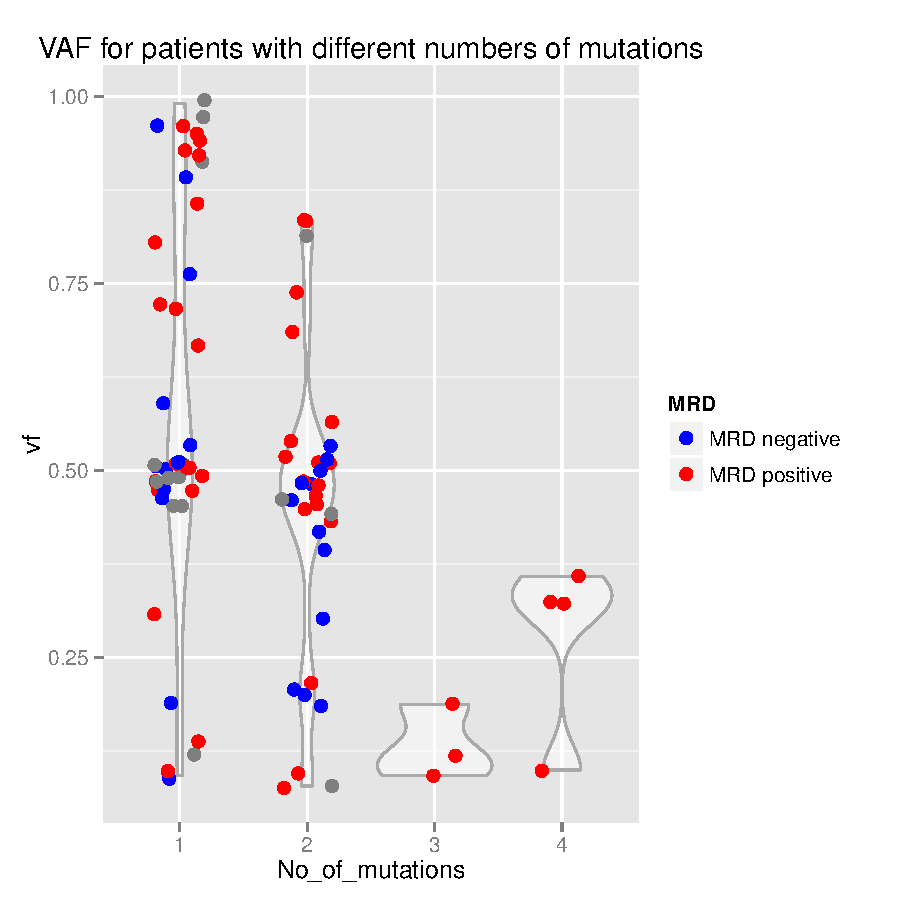
\includegraphics{ATM_VAF-007}
\\Surprisingly, there seems to be much clearer clustering in the patients with only one mutation.\\
NExt, we want to focus on the patients with two mutations and see if there is really a clear separation in the VAFs. To do this, we first select all the patients with two mutations. Then we rank their VAF and assign a lower and a higher VAF. 
We check if low and high VAF are correlated:\\
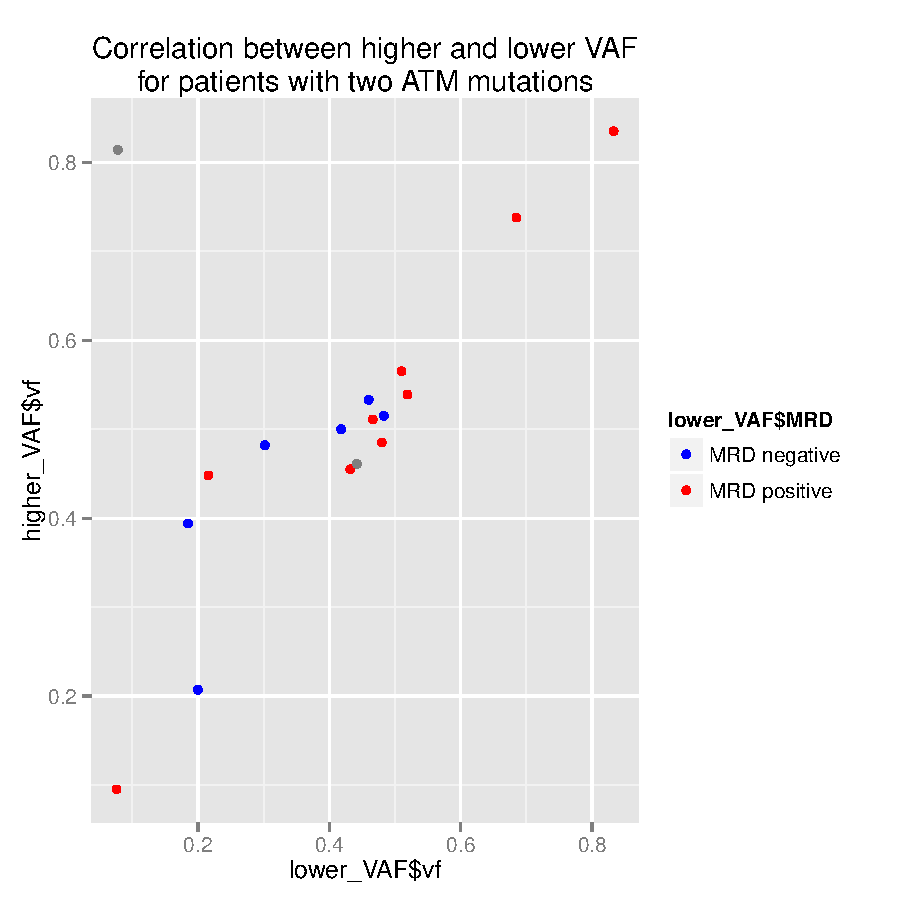
\includegraphics{ATM_VAF-009}
\begin{Schunk}
\begin{Soutput}
	Pearson's product-moment correlation

data:  lower_VAF$vf and higher_VAF$vf
t = 2.7684, df = 15, p-value = 0.01435
alternative hypothesis: true correlation is not equal to 0
95 percent confidence interval:
 0.1399974 0.8301341
sample estimates:
      cor 
0.5815127 
\end{Soutput}
\end{Schunk}
\\We can see that there is a clear correlation between the low and the high VAF of patients with two mutations. In other words, there is not much variation going on WITHIN a patient. Both mutations occur at nearly the same frequencies (except for one outlier). Now we want to see how much variance we find BETWEEN the two mutations.\\
By connecting each individuals VAFs with a line, we can see the slope that is created by each individual. If the slope is relatively flat, there is no difference between the groups. If we can detect a slope, we can say that the lower and higher vafs generally differ from each other, while correcting for within patient variation. The paired wilcoxon test checks if this slope is different from 0. Addmitetly, this is a bit of an artificial approach because we SORTED the VAFs in the first place.\\

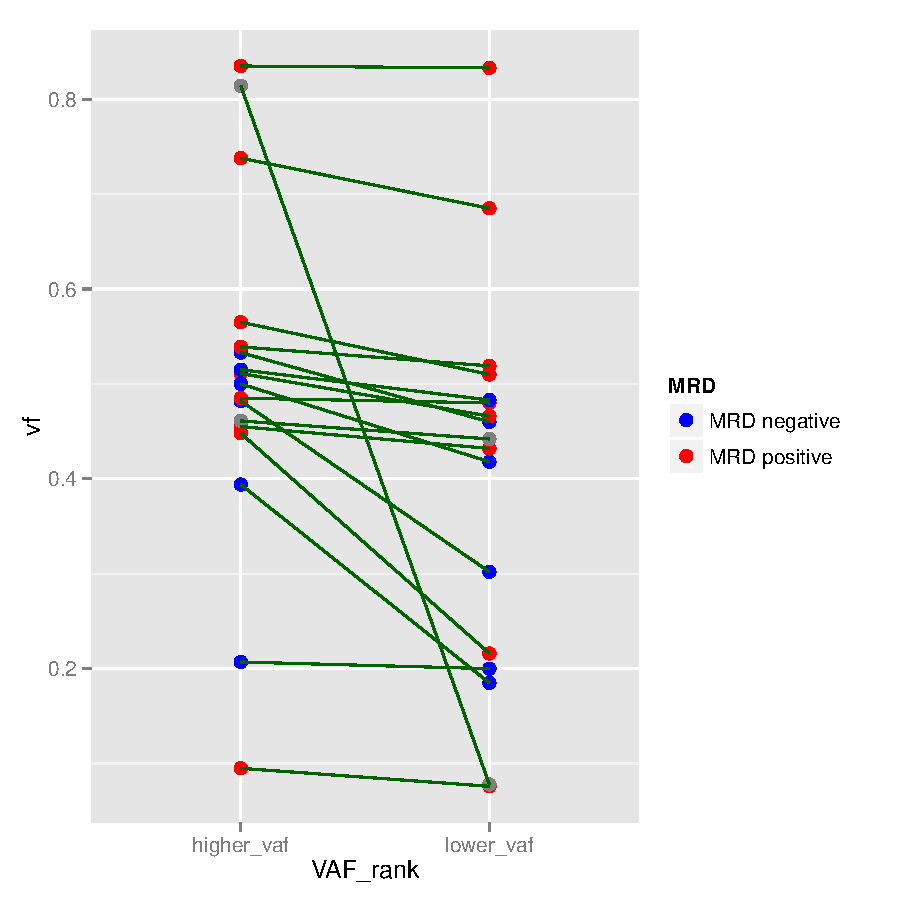
\includegraphics{ATM_VAF-011}
\begin{Schunk}
\begin{Soutput}
	Paired t-test

data:  lower_VAF$vf and higher_VAF$vf
t = -2.4455, df = 16, p-value = 0.02641
alternative hypothesis: true difference in means is not equal to 0
95 percent confidence interval:
 -0.19678856 -0.01403497
sample estimates:
mean of the differences 
             -0.1054118 
\end{Soutput}
\end{Schunk}
\\I removed the outlier here:\\
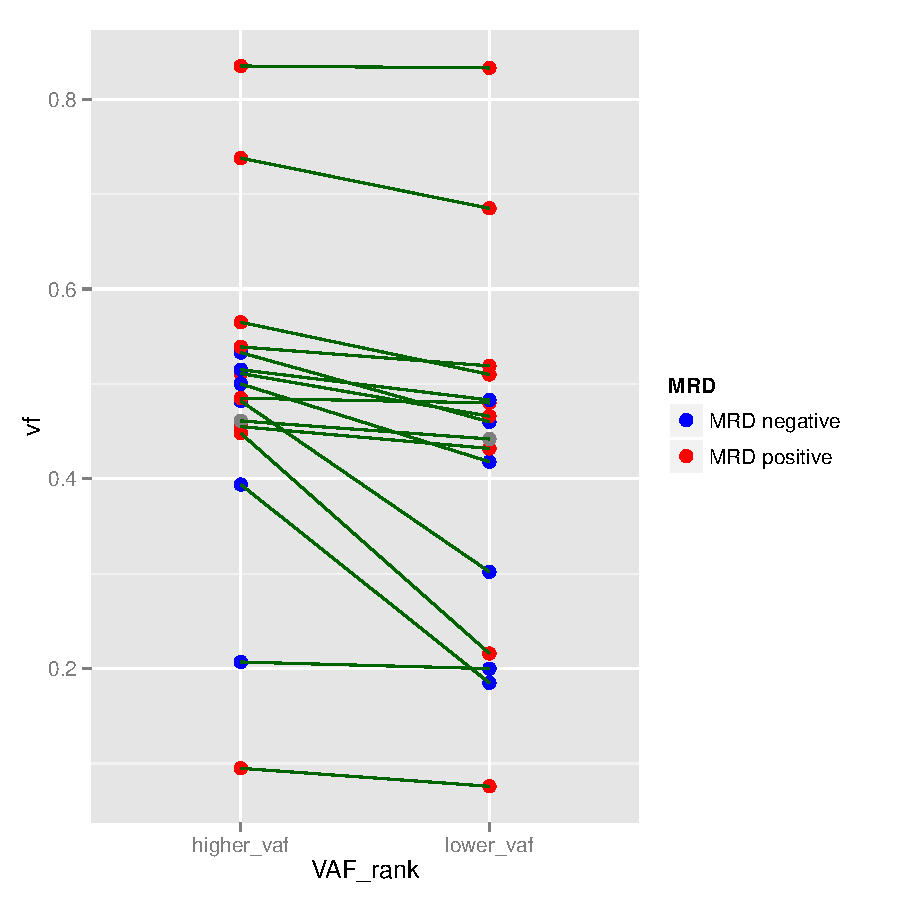
\includegraphics{ATM_VAF-014}
\begin{Schunk}
\begin{Soutput}
	Paired t-test

data:  lower_VAF_out$vf and higher_VAF_out$vf
t = -3.5517, df = 15, p-value = 0.002899
alternative hypothesis: true difference in means is not equal to 0
95 percent confidence interval:
 -0.10560761 -0.02639239
sample estimates:
mean of the differences 
                 -0.066 
\end{Soutput}
\end{Schunk}
\\We can see that the difference is significant as expected, but it is rather small (-0.06). Both the correlation between low and high VAF and relatively small difference allows us to use the mean(VAF) for each sample for a final comparison.\\
\section*{Comparison of mean(VAF) in samples with 1 or >1 ATM mutation}
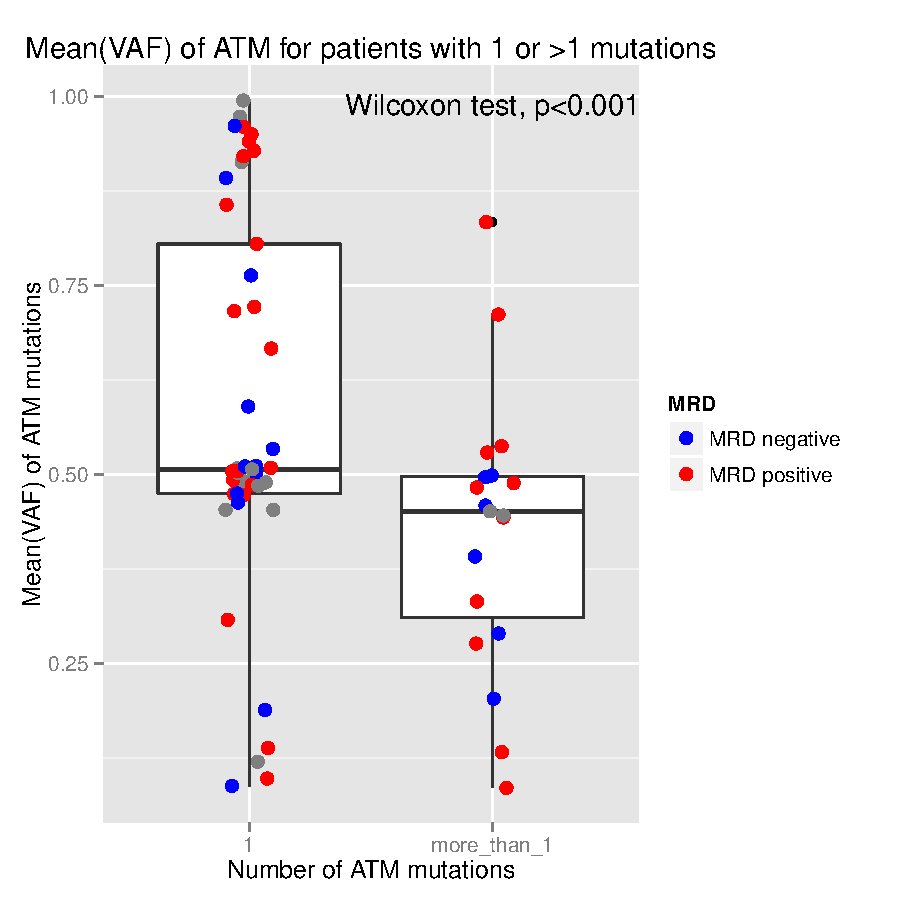
\includegraphics{ATM_VAF-016}
\\We use a simple ANOVA-like approach to see if the mean(vaf) is influenced by a combination of "Numer of mutations" and "MRD": Again, we see that only number of mutations has an effect on mean(vaf).\emph{(p adj=0.02)}\\
\begin{Schunk}
\begin{Soutput}
  Tukey multiple comparisons of means
    95% family-wise confidence level

Fit: aov(formula = mean_vaf ~ Binary_No_of_mutation * MRD, data = duplicate_atm)

$Binary_No_of_mutation
                    diff        lwr         upr     p adj
more_than_1-1 -0.1659724 -0.3094049 -0.02253987 0.0242941

$MRD
                                diff         lwr     upr     p adj
MRD positive-MRD negative 0.07400826 -0.06597347 0.21399 0.2927852

$`Binary_No_of_mutation:MRD`
                                                         diff         lwr
more_than_1:MRD negative-1:MRD negative           -0.14739103 -0.46139153
1:MRD positive-1:MRD negative                      0.08539231 -0.14126574
more_than_1:MRD positive-1:MRD negative           -0.09612587 -0.35676430
1:MRD positive-more_than_1:MRD negative            0.23278333 -0.06335654
more_than_1:MRD positive-more_than_1:MRD negative  0.05126515 -0.27162391
more_than_1:MRD positive-1:MRD positive           -0.18151818 -0.42033799
                                                         upr     p adj
more_than_1:MRD negative-1:MRD negative           0.16660947 0.5980908
1:MRD positive-1:MRD negative                     0.31205035 0.7477286
more_than_1:MRD positive-1:MRD negative           0.16451255 0.7597328
1:MRD positive-more_than_1:MRD negative           0.52892321 0.1699016
more_than_1:MRD positive-more_than_1:MRD negative 0.37415421 0.9742280
more_than_1:MRD positive-1:MRD positive           0.05730163 0.1934759
\end{Soutput}
\end{Schunk}

\section*{Conclusion}
The strongest effect is that VAFs of patients with more than one mutations are remarkably similar and do not cluster clearly into two groups. It almost seems as if they co-occur. Are they defined as being in different clones? If so, I strongly suggest to check on this as they may be from the same clone.\\
We can also conclude that patients with more than one mutation generally have lower VAF.\\
\\
\textbf{Possible explanation:}\\
One reason for this finding could be the following: Two mutations occureing at similar vafs could belong to the same clone. As the event of having two mutation is much rarer than having only one mutation, their vaf is generally lower.\\
\\
\textbf{Outlook:}\\
As the difference is quite clear cut, could that allow us to calculate a mutation rate for ATM mutations?\\
Can we have a look at vafs of other genes?\\
We still have the length of our mutations somewhere stored and have not used them for any analysis. We could check if VAFs are related to mutation length.





\Sconcordance{concordance:ATM_VAF.tex:ATM_VAF.Rnw:%
1 12 1 1 0 7 1 1 24 6 2 1 3 5 0 1 1 6 0 3 2 2 1 1 4 1 2 2 1 1 10 1 3 13 %
0 1 2 2 1 1 4 1 3 13 0 1 2 1 6 1 5 13 0 1 2 1 1 1 9 1 5 1 3 31 0 1 2 20 %
1}



\end{document}
